\documentclass{article}
\usepackage{hyperref}
\usepackage{amsmath}
\usepackage[pdftex]{graphicx}
\usepackage{url}
\usepackage{enumerate}

\hypersetup{
colorlinks=true,
linkcolor=blue,
citecolor=blue,
urlcolor=blue,
}

\author{Rohit Kumar \\UCLA ID: 203884129}
\title{Data Mining Chess Games \\ CS 249: Term Project, Winter 2011}
\begin{document}

\maketitle


\section{Introduction}
\label{sec:intro}
The Free Internet Chess Server (FICS) \footnote{http://www.freechess.org} maintains an extensive set of chess games in its database. The data set contains games from 1999 to 2011 and includes players of all kinds of ratings -- from the very beginner, to grand masters, to computers. Apart from the traditional chess games, people also play chess variants on the server. For example: suicide chess, losers, crazyhouse etc. The data for each game is captured as a Portable Game Notation (PGN) \cite{wiki:pgn} file and contains information regarding the moves played, the players names, their rating, time controls used and the result. \\

As of this writing the FICS chess database contains game records for over 130,000,000 chess games, played by over 300,000 humans and 1,400 computers. This project aims at finding interesting patterns in the FICS chess data set.

\section{Data Acquisition}

\subsection{PGN Parser}

As mentioned in Section~\ref{sec:intro}, the games in the FICS
database are stored in the PGN file format. PGN is a standard way for
storing chess games. It was designed for ease of viewing of chess
games and not for querying ~\cite{spec:pgn}. Thus to extract meaningful information out of the database, the PGN files need to be parsed.

PGN is a text based format and looks in some ways similar to the Windows INI file format. An example file, is shown in Figure~\ref{fig:pgn}

\begin{figure}[htp]
\begin{center}
\begin{verbatim}
[Event "FICS rated blitz game"]
[Site "FICS"]
[FICSGamesDBGameNo "273548609"]
[White "tirsa"]
[Black "EyeLikePie"]
[WhiteElo "1015"]
[BlackElo "1083"]
[TimeControl "180+0"]
[Date "2011.03.01"]
[Time "18:00:00"]
[WhiteClock "0:03:00.000"]
[BlackClock "0:03:00.000"]
[ECO "C57"]
[PlyCount "33"]
[Result "1-0"]


1. e4 {[%emt 0.0]} e5 {[%emt 0.0]} 
2. Nf3 {[%emt 0.57]} Nc6 {[%emt 0.39]} 
3. Bc4 {[%emt 0.692]} Nf6 {[%emt 2.781]} 
4. Ng5 {[%emt 1.812]} d5 {[%emt 7.405]} 
5. exd5 {[%emt 1.79]} Nxd5 {[%emt 0.859]} 
6. Qf3 {[%emt 6.995]} Qxg5 {[%emt 11.124]} 
7. Bxd5 {[%emt 2.384]} f6 {[%emt 14.233]} 
8. Bxc6+ {[%emt 3.291]} bxc6 {[%emt 1.796]} 
9. d3 {[%emt 1.242]} Bb4+ {[%emt 1.719]} 
10. Nc3 {[%emt 3.945]} Bxc3+ {[%emt 4.969]} 
11. bxc3 {[%emt 1.391]} Qg6 {[%emt 4.593]} 
12. O-O {[%emt 5.834]} Bg4 {[%emt 0.672]} 
13. Qxc6+ {[%emt 4.156]} Kf7 {[%emt 3.172]} 
14. Qxc7+ {[%emt 0.899]} Ke6 {[%emt 2.343]} 
15. Qc4+ {[%emt 1.71]} Kf5 {[%emt 4.203]} 
16. f3 {[%emt 0.733]} Bxf3 {[%emt 1.828]} 
17. Rxf3# {[%emt 3.97]} {Black checkmated} 1-0

\end{verbatim}
\end{center}

\caption{Example PGN File.}
\label{fig:pgn}
\end{figure}

Each PGN file can have details regarding more than one game. A game contains some meta information like the player information, their ratings, the time controls used, which is followed by the actual moves played by the players.\\

The meta information is stored as key-value players and are the fields enclosed within '[' and ']' in Figure~\ref{fig:pgn}. The moves come after that and are prefixed with numbers. The white player's move is listed first, followed by black. The moves are denoted using the Standard Algebraic Chess Notation~\cite{wiki:san}. \\

The PGN parser extracts both the meta information and the moves from the PGN file. The contents of the entire PGN file is stored within a \verb=PgnDatabase= class. The \verb=PgnDatabase= class contains a list of \verb=PgnGame= instances.

\subsection{Player Statistics}
\label{sec:pstats}
The PGN database only gives details regarding individual games played on the FICS server. It doesn't give us individual player statistics. These were gathered by executing a command on the FICS server called \verb=finger=. 

The \verb=finger= command lists a player's details such as, their rating, number of games played, won, lost, etc. An example output of running the command \verb="finger roxtar"= on the FICS server is shown in Figure~\ref{fig:finger}

\begin{figure}[htp]
\begin{verbatim}
>finger roxtar

Finger of roxtar:

On for: 29 mins   Idle: 0 secs

          rating     RD      win    loss    draw   total   best
Blitz      1044     34.2     670     693      30    1393   1161 (04-Apr-2008)
Standard   1178    350.0       3       5       0       8
Lightning  1004    289.5       5      10       0      15
Bughouse   1323    350.0       2       4       0       6
Crazyhouse 1388    166.7      16      26       0      42   1272 (27-Feb-2005)
Suicide    1705    173.5     152     222       6     380   1654 (08-Dec-2004)
Losers     1877    350.0       7       6       0      13


Timeseal 1 : On

 1: I prefer 2 12 or 10 0.
 2: No takebacks asked or given.
 3: The variants which I like to play include suicide and crazyhouse.
\end{verbatim}
\caption{Example Finger Output}
\label{fig:finger}
\end{figure}

\pagebreak

To execute the \verb=finger= command on the server a Perl script was written, which would telnet to the FICS server, run the command and return the output. The output was then filtered to obtain the player statistics in CSV format. \\

The FICS website or server doesn't provide a means to extract a list of all user names in the system. So instead, a PGN file containing 5000 games was downloaded for each month between March 2010 to March 2011 and the statistics for all users who participated in those games was extracted. 

\section{Data Analysis}

\subsection{Exploring Ratings}
The FICS server has got a rating system based on the Glicko system~\cite{spec:glicko}. Each player has a rating which is a number ranging between 600-3000. The higher the rating, the better the player. The Glicko rating system has another factor called \textsl{Ratings Deviation(RD)}, which measures the accuracy of the rating. The lower the Ratings Deviation (RD), the more accurate is the rating of the player.\\

In addition to this, the FICS server allows to users to play at a pace of their own choice. This leads to three varieties of time controls in regular chess: lightning, blitz and standard. Lighting being the fastest, with games finishing in under 6 minutes total, and standard being the slowest. For each of these different time controls, the user has different ratings, i.e a user's blitz rating will not be influenced by any of the lightning games which she plays and vice-versa.Time controls which fall under the blitz category are the most popular.\\

\begin{figure} [htp]
\begin{center}
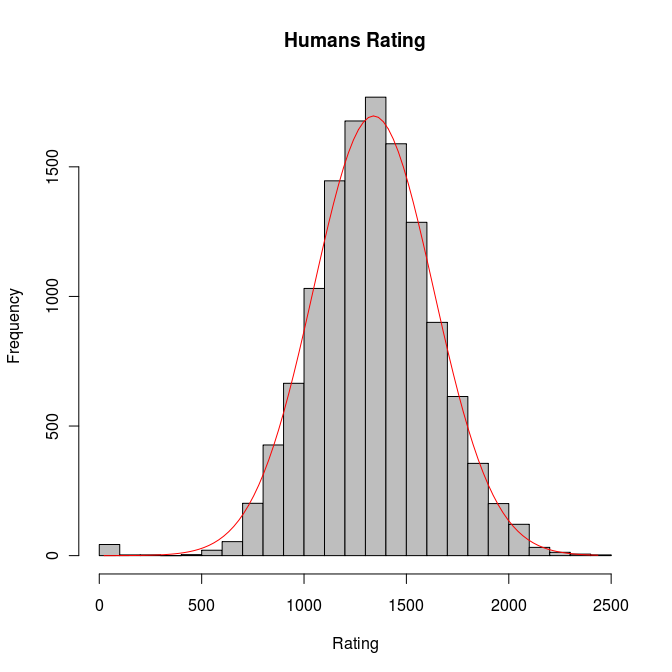
\includegraphics[width=3in]{humans_rating.png}
\end{center}
\caption{Distribution of Human Players' Rating}
\label{fig:humanrating}
\end{figure}


To explore the ratings of the players on FICS, the finger statistics were downloaded and transformed into a CSV format as described in section~\ref{sec:pstats}. This was done separately for human players and computer programs. On plotting the histogram of the human ratings, for blitz games, we observe that the ratings have normal distribution (Figure \ref{fig:humanrating}). With the mean $\bar{x}_{hr} = 1339.560$ and standard deviation $\sigma_{hr} = 293.12$\footnote{The author's own rating is below average at 1084}.\\

\begin{figure} [htp]
\begin{center}
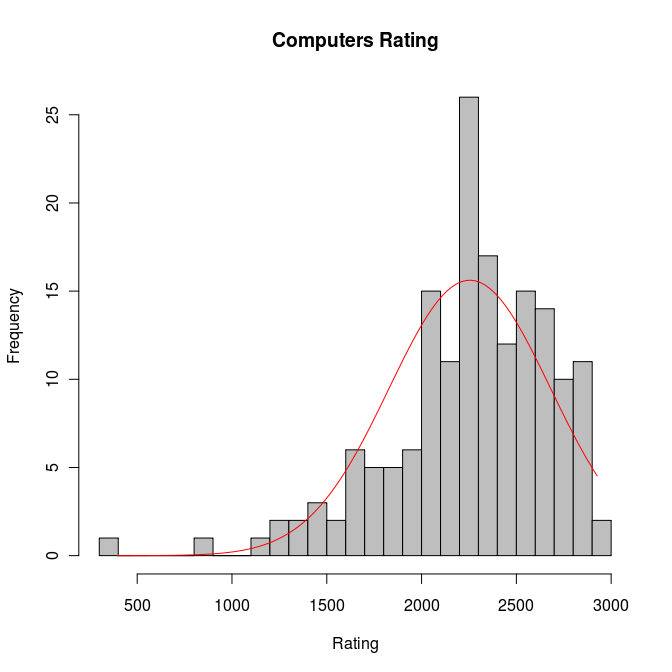
\includegraphics[width=3in]{computers_rating.png}
\end{center}
\caption{Distribution of Computers' Rating}
\label{fig:comprating}
\end{figure}


The computer accounts which are present on the FICS server run chess programs. These programs are either commercially available programs like Fritz~\cite{web:fritz}, or are open source, like Crafty~\cite{web:crafty} or mscp~\cite{web:mscp}. Apart from the kind of program running, the computers running them differ in hardware. The hardware's capabilities also influence the chess program's strength. With faster hardware we would expect the program to be able to search deeper in the tree. Due to these two factors, namely difference in programs and difference in hardware, we would expect to see some variance in the ratings of the computers. At the same time, as these programs are playing against regular human beings (and not grand masters) we expect that their mean rating will be higher than that of humans. \\

The list of computers operating on the FICS server was available readily. The same procedure was applied to obtain their statistics. The computer blitz ratings histogram differ significantly from the human ratings. We see in Figure \ref{fig:comprating} that the computer ratings do not seem to follow a normal distribution. Most computers are rated higher than 2000. To compare this against humans, $79.6\%$ of computers are rated above 2000, whereas only $1.44\%$ of humans cross that level. The mean rating for computers is $\bar{x}_{cr} = 2254.479$ with standard deviation $\sigma_{cr} = 426.53$. One thing to note though is that the number of active computer players is far less than human players.\\



\subsection{Game Totals}

A related statistic is the number of games a particular user has played. One could conjecture that human players would have played lesser number of games as compared to the computers on the server. The totals for the blitz games played, were plotted for humans and computers (Figure~\ref{fig:gametotals}). The computer which has played the highest number of blitz games is {\sl mscp(C)} and the human is a user named {\sl gianti}. What's surprising is that {\sl mscp(C)} has played over 1 million games, which is 10 times the number of games which {\sl gianti} has played.\\


\begin{figure} [htp]
\begin{center}
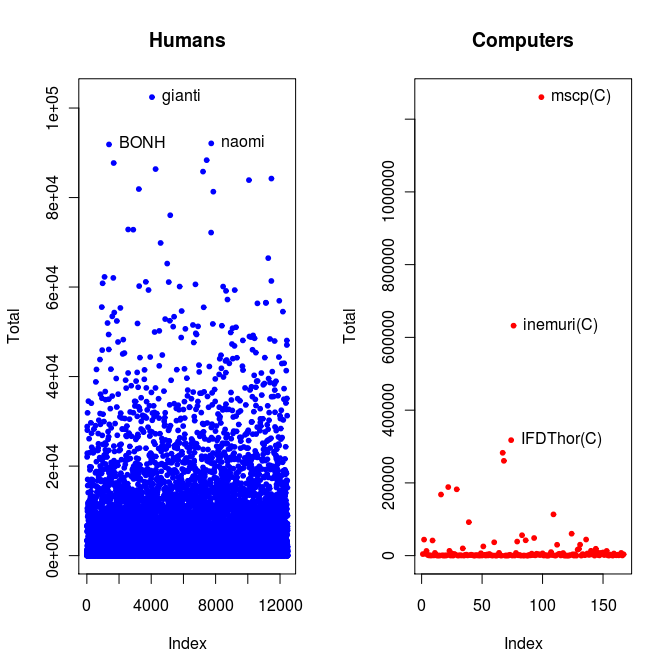
\includegraphics[width=3in]{game_totals.png}
\end{center}
\caption{Blitz Game Totals for Humans and Computers}
\label{fig:gametotals}
\end{figure}



One might postulate that a human player's rating is correlated to the number of games she has played. With the assumption that a player will learn and improve over time. This though is found to be not true. If we plot the player's rating against her ratings deviation (which is a measure of the how frequently a user plays games and the accuracy of her rating) and the total number of games played, we find that there is no such correlation (Figure~\ref{fig:ratingsrdtotal}).\\

\begin{figure} [htp]
\begin{center}
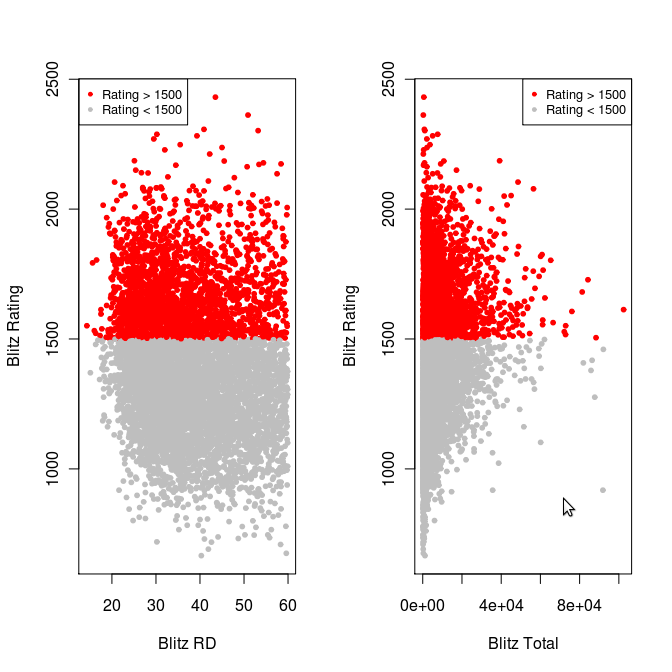
\includegraphics[width=3in]{ratings_rd_total.png}
\end{center}
\caption{Blitz Game Totals for Humans and Computers}
\label{fig:ratingsrdtotal}
\end{figure}

\begin{table}[htp]
\begin{center}
\begin{tabular}{|c|c|c|c|c|c|c|}
\hline

- & Rating & RD & Won & Lost & Drawn & Total \\
\hline
Rating & 1.00 & -0.16 & 0.28 & 0.18 & 0.31 & 0.24\\
\hline
RD & -0.16 & 1.00 & -0.35 & -0.37 & -0.33 & -0.37\\
\hline
Won & 0.28 & -0.35 & 1.00 & 0.89 & 0.89 & 0.97\\
\hline
Lost & 0.18 & -0.37 & 0.89 & 1.00 & 0.88 & 0.97\\
\hline
Drawn & 0.31 & -0.33 & 0.89 & 0.88 & 1.00 & 0.92\\
\hline
Total & 0.24 & -0.37 & 0.97 & 0.97 & 0.92 & 1.00\\
\hline
\end{tabular}
\end{center}
\caption{Correlation Matrix for Player Statistics}
\label{tab:playercor}
\end{table}



This is confirmed when we see the correlation matrix for the player statistics in Table~\ref{tab:playercor}. We can see that in the row for ``Rating'' almost all columns are below 0.4 and above 0.1. We see strong correlation between the ``Total'' and the ``Won'', ``Lost'' and ``Drawn'' columns, but that's expected because ``Total'' is the sum of those three columns. What's interesting though is the ``Won'' row, where we find that the number of wins is strongly correlated to the number of ``Lost'' and ``Drawn'' games. \\



Another thing which can be noticed is that most computers have totals below 200,000 games, whereas for humans this number is 60,000. We considered points above these numbers as outliers and plotted the histogram for the totals. We find that the distribution for humans follows a power law (Figure~\ref{fig:totalsdistr}). The distribution for the computers though is not as beautiful (Figure~\ref{fig:totalsdistr}).\\

\begin{figure} [htp]
\begin{center}
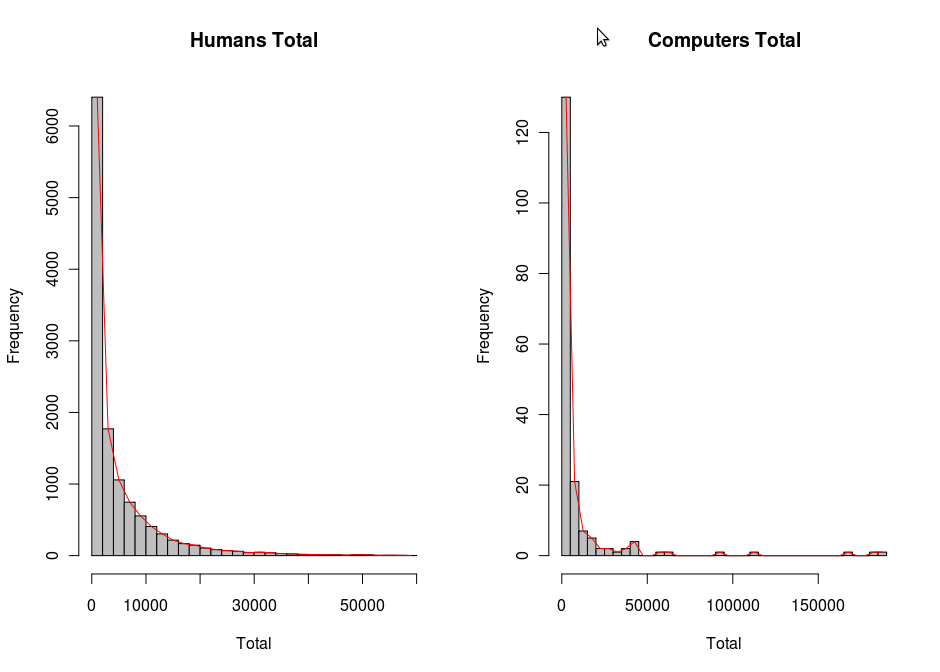
\includegraphics[width=3in]{totals_distr.png}
\end{center}
\caption{The Distribution of Total Games for Humans and Computers}
\label{fig:totalsdistr}
\end{figure}

\clearpage
\subsection{Opening Strategies}
The initial moves played in a chess game constitute of what is known as the ``Opening'' of a game. There are various opening strategies each with its strength and weaknesses. Although the first move is played by White, the opening relies open Black's response.\\

The standard way of categorizing chess openings is to use Encyclopaedia of Chess Openings or ECO codes. The ECO codes are categoriezed into five sub-divisions labeled from ``A'' to ``E''. Each sub-division in turn has 100 sub-categories~\cite{wiki:eco}.\\

In all of the games played on FICS, these ECO codes are recorded in the PGN files as a tag with key ``ECO''. This saves us the trouble of deciphering the ECO codes from the moves played. We can plot the frequency of the most popular openings as a barchart. This is shown in Figure~\ref{fig:ecobar}.

\begin{figure} [htp]
\begin{center}
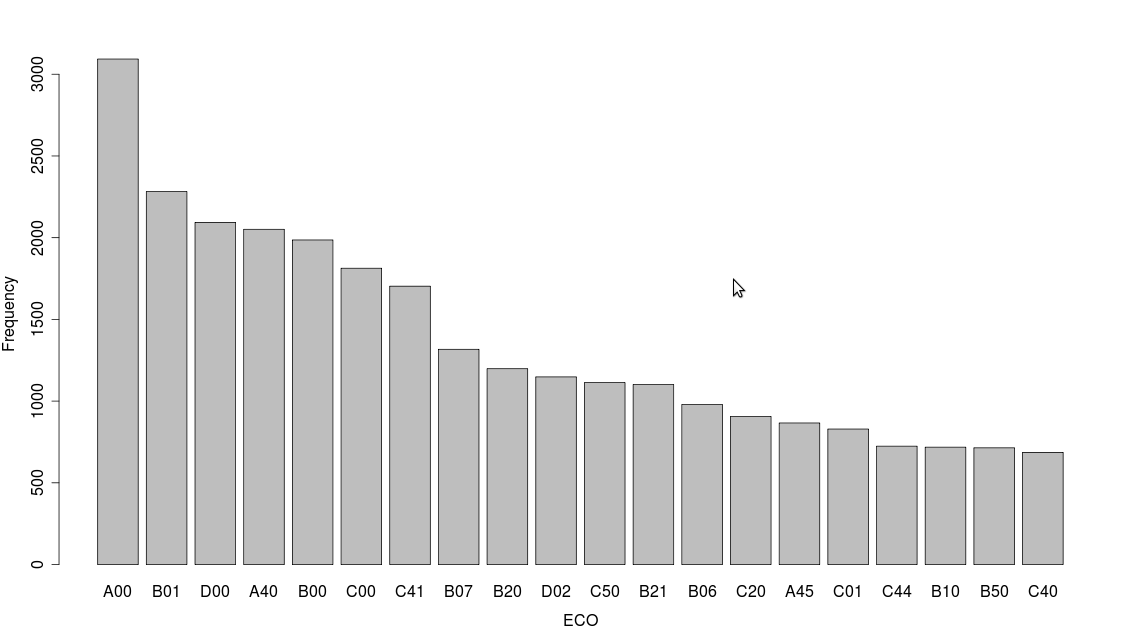
\includegraphics[width=5in]{eco_bar.png}
\end{center}
\caption{Bar-plot Showing the 20 most popular Openings}
\label{fig:ecobar}
\end{figure}

Surprisingly the most popular opening is the A00 opening. A00 is the ``uncommon opening'' , which as the name suggests should be ``uncommon'' but is in fact the most common. The 2nd opening, B01 is the Scandinavian opening and starts with the {\bf 1. e4 d5} (white moves the King's pawn two steps, to which Black counters by moving her Queen's pawn two steps). The bar plot of course shows openings across all ratings. On changing the ratings and plotting we would expect to see a difference in the frequency of the ratings. This is found to be true as seen in Figure~\ref{fig:ecobarcomp}

\begin{figure} [htp]
\begin{center}
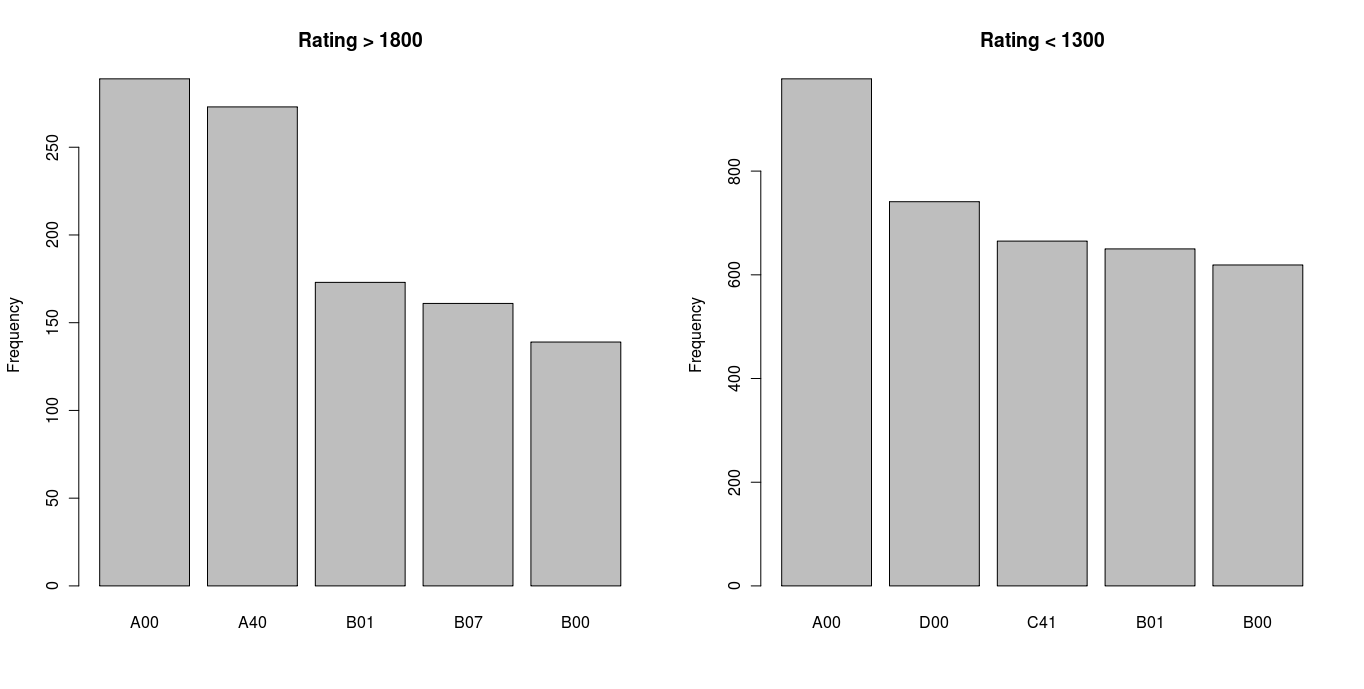
\includegraphics[width=5in]{eco_bar_comp.png}
\end{center}
\caption{Top Five Openings for Above Average and Below Average Players}
\label{fig:ecobarcomp}
\end{figure}


\subsection{Frequent Pattern Mining}
Pattern Mining deals with finding interesting patterns in an itemset. This includes finding associations, sequences, clusters, etc. Finding out association rules was first used in the analysis of market transactions. It was first presented in 1993 by Agrawal~\cite{paper:agrawal}. The basics of pattern mining with specific focus on association rules is presented in the following sub-section.


\subsubsection{Definitions}
The definitions presented in this section are from the report ``A Survey on Frequent Pattern Mining'', by Bart Goethals~\cite{report:patternmining}.\\

Let $I$ be a set of items. A set $X = \{i_1, ... i_k\} \subseteq I$ is called an {\sl itemset}. \\

A {\sl transaction} over $I$ is a couple $T = (tid, I)$ where {\sl tid} is the transaction identifier and $I$ is an itemset. A {\sl transaction database} $D$ over $I$ is a set of transactions over $I$. \\

The {\sl cover} of an itemset $X$ in $D$ consist of the set of transaction identifiers of transactions in $D$ that support $X$:

\[cover(X, D) := \{tid | (tid, I) \in D, X \subseteq I\}. \]

The {\sl support} of an itemset $X$ in $D$ is the number of transactions in the cover of $X$ in $D$:

\[support(X, D) := |cover(X,D)|.\]

An itemset is called {\sl frequent} if its support is no less than a given absolute {\sl minimal support threshold $\sigma_{abs}$}, with  $0 \le \sigma_{abs} \le |D|$.

{\bf Definition 1.} Let $D$ be a transaction database over a set of items $I$, and $\sigma$ a minimal support threshold. The collection of frequent itemsets in $D$ with respect to $\sigma$ is denoted by: 

\[F(D,\sigma) := \{X \subseteq I | support(X, D) \ge \sigma\}.\]

{\bf Problem 1. (Itemset Mining)} Given a set of items $I$, a transaction database $D$ over $I$, and minimal support threshold $\sigma$, find $F(D, \sigma)$.\\

In practice we are not only interested in the set of itemsets $F$, but also
in the actual supports of these itemsets.\\

An association rule is an expression of the form $X \Rightarrow Y$ ,
where $X$ and $Y$ are itemsets, and $X \cap Y = \{\}$. Such a rule
expresses the association that if a transaction contains all items in
$X$, then that transaction also contains all items in $Y$. $X$ is called
the body or antecedent, and $Y$ is called the head or consequent of the
rule.\\

The support of an association rule $X \Rightarrow Y$ in $D$, is the
support of $X \cup Y$ in $D$. An association rule is called
frequent if its support exceeds a given minimal support
(frequency) threshold $\sigma_{abs}$. \\

The confidence or accuracy of an association rule $X \Rightarrow Y$ in
$D$ is the conditional probability of having $Y$ contained in a
transaction, given that $X$ is contained in that transaction:

\[confidence(X \Rightarrow Y, D) := P(Y|X) = \frac{support(X \cup Y, D)}{support(X,D)}\]

The rule is called confident if $P(Y|X)$ exceeds a given minimal confidence threshold $\gamma$, with $0 \le \gamma \le 1$. \\

{\bf Definition 2.} Let $D$ be a transaction database over a set of items $I$, $\sigma$ a minimal support threshold, and $\gamma$ a minimal confidence threshold. The collection of frequent and confident association rules with respect to $\sigma$ and $\gamma$ is denoted by:

\begin{align*}
R(D, \sigma, \gamma) := \{X \Rightarrow Y | X, Y \subseteq I, \\
X \cap Y = \{\}, \\X \cup Y \in F(D, \sigma),\\ confidence(X \Rightarrow Y, D) \ge \gamma\}
\end{align*}\\


{\bf Problem 2. (Association Rule Mining)} Given a set of items $I$, a transaction database $D$ over $I$, and minimal support and confidence thresholds $\sigma$ and $\gamma$, find $R(D, \sigma, \gamma)$. \\

For a more thorough discussion on itemset and association rule mining please see~\cite{report:patternmining}.\\

\subsubsection{Association Mining in R}

The packages {\sl arules}~\cite{r:arules} and {\sl arulesSequences}~\cite{r:arulesseq} are two libraries which can be used for itemset and association mining in R. They can be installed using the standard \verb=install.packages= command. These packages required R 2.11 or greater.\\

The {\sl arules} package provides functions to read in transactions
and perform association mining using a number of algorithms, like
apriori, eclat, FP-growth etc.\\

To read transaction data, the \verb=read.transactions= method can be
used. The method takes the name of a file which contains transaction
data. The transaction data are separated using a delimiter. The
\verb=read.transactions= method returns a transaction object. One can
get information about an item's support values from the transaction
object. The transaction object can also be used to deduct association
rules by passing it to the \verb=apriori= method.

\subsection{Pattern Mining Chess Games}
One way to think of chess games is to think of the individual moves
played in a game as an itemset chosen from all possible moves. To use
the frequency pattern mining terminology, individual games can be
thought of as a transaction, where moves are items. The entire game
database is analogous to the transaction database. \\

Thus, it is possible to use pattern mining to discover patterns in
chess games. We would expect to see high support and confidence values
for rules which represent the opening moves. This would be because
most chess games start of with standard opening moves. But at the same
time, trying to discover interesting association rules is hard, due to
the following reasons.

\begin{enumerate}
\item The number of games present in the game database (or more exactly the portion of the database which was downloaded) is quite large. 

\item The number of individual moves played per game is large.

\item We don't clearly know what we are looking for or what we mean by  ``interesting.''

\end{enumerate}

\subsection{Weeding out Cheaters}
As mentioned before the FICS chess server hosts many chess programs. Many of these programs are hobby projects and aren't highly rated. Amongst these there are computers which do not {\sl learn} from their previous games. Thus it is possible for a human player to exploit a particular weakness in a computer's game by playing the same moves from a previously won game. By doing this, the human can easily increase her rating. The server policy explicitly states that \cite{web:ficspolicy}
\begin{quote}
{\sl 13. It is against server policy, when playing against computer accounts, to play the same line repeatedly (e.g. to inflate your rating).}
\end{quote}

Despite that, there is no strict checking in place to find humans who do this. Using pattern mining techniques, we could find if such cheaters exist.\\

If someone is inflating their rating by playing similar moves repeatedly, we would expect such moves to have low support, but  high confidence values. We assume that in most games against computers humans don't cheat, but people who cheat, do so repeatedly. \\

The last 10000 games of three computer programs were downloaded. These programs were {\sl mscp, inemuri and IFDThor}. They are the top three amongst the computers which have played the most number of games. Half the games consisted of plays where the computer was playing White and the other half Black. The game database PGN files were parsed and the moves were extracted into a CSV file format which would be understandable by the \verb=read.transactions= function. Each game was listed as a sequence of comma separated moves on each line of the file. The first item on each line is the game ID (Figure~\ref{fig:movecsv}).\\

\begin{figure}[htp]

\begin{verbatim}
274021904, fxg4,Rd4, Nf2,Rxd3, Rxd3,f5, Rxe3,Qc5, Rxe6,fxg4, Re8,Qxh5
274021494, b6,e5, b7,Kd6, b8=Q+,Ke6, Nc5+,Kd5, Nab3,Ne6, Nxe6,Kxe6, Ke2
274021332, Rxb4,a2, Ra4,Kc5, Rxa2,Kc4, Ra4+,Kd5, Rd4+,Ke6, Rxd3,Kf5, Ke3
274021097, Kh3,Rb2, Rg5,g6, Re5,h6, Rxe6+,Kb5, Rce4,g5, fxg5,hxg5, hxg5
274019453, b6,Nd2+, Kd5,Nf3, b7,Nd4, b8=Q,Nf3, Qd6+,Kg7, Qe7,Ne1, Qxf7+
274018954, Rxe8,Rxe8, Ke6,a5, d7,Rxe7+, Kxe7,a4, d8=Q,Kh6, Qb6+,g6, Qa5
\end{verbatim}
\caption{Comma Separated Move File}
\label{fig:movecsv}
\end{figure}


On applying the association rule mining function \verb=apriori= we found that there were a large number of association rules generated. Looking at the rules, it was found that a number of rules corresponded to the opening moves of the game and as many games share the same opening they had high associativity. To cut down on the number of association rules, rather than looking at all the moves of a game, we could only look at the last 10 moves. Also as we were looking for cheaters, we needed only look at those games where the computer lost.\\


After filtering the games, we were able to cut down on the number of association rules generated. We also needed to play around with the support and confidence values to obtain a manageable number of rules. A listing of the top 10 rules for the computer account {\sl inemuri} is listed in Figure~\ref{fig:inemuriwhite}.

\begin{figure}[htp]
\begin{verbatim}
       lhs        rhs        support confidence     lift
    1  { Nf3}  => { c3}   0.10042008  0.6107056 3.200123
    2  { bxa3} => { c3}   0.08321664  0.9742389 5.105053
    3  { Bxf6} => {f6}    0.08321664  0.8404040 8.189434
    4  {f6}    => { Bxf6} 0.08321664  0.8109162 8.189434
    5  { Bxf6} => { Nf3}  0.08321664  0.8404040 5.110924
    6  { bxa3} => {a3}    0.08261652  0.9672131 8.557696
    7  {a3}    => { bxa3} 0.08261652  0.7309735 8.557696
    8  {f6}    => { Nf3}  0.08261652  0.8050682 4.896029
    9  {a3}    => { c3}   0.08201640  0.7256637 3.802508
    10 { Bg5}  => { Bxf6} 0.07781556  0.9373494 9.466282
\end{verbatim}

\caption{Top 10 Association Rules for inemuri playing White}
\label{fig:inemuriwhite}
\end{figure}

We can see that the rule $\{bxa3\} \Rightarrow \{c3\}$ has the highest confidence measure (0.97). When this move sequence was searched for {\sl inemuri's} game database it was found to be heavily repeated. The exact move sequence being:

\begin{quote}
\begin{verbatim}
Nf3, a3 
Bg5, f6
Bxf6, Qxf6
bxa3, Bxa3
Bxh7+, Kxh7
c3, Bf5+
Rd3, Bxd3+  {White resigns} 0-1
\end{verbatim}
\end{quote}

There were similar repeated move sequences found when {\sl inemuri} played black. For {\sl mscp} and {\sl IFDThor} we were unable to find such moves and that could be one reason why both those programs are rated higher than {\sl inemuri} \footnote{mscp: 1636, IFDThor: 1638, Inemuri: 1337}.

\section{Conclusion and Lessons Learnt}

Mining the chess game database was an enjoyable exercise. There were many thing which the were discovered which weren't evident at the onset. A major portion of the time was spent in trying to acquire the data and cleanse it. One such challenge was in acquiring the player statistics data. The initial method to obtain player statistics used the FICS website. A script would run in a loop and repeatedly query the website for the statistics, which would then be downloaded. This method though generated a lot of requests. In response, the server administrators blocked my IP address from accessing the web page, thinking it was a DoS attack. On contacting the server administrators, they suggested that a better way would be to make the script directly telnet to the server and then download the data. \\

R was found to be a powerful tool. Learning parts of it though is hard.  When searching through Google many times the search engine would just drop the term ``R'' and search for the rest of the keywords.\\ 

Many of the techniques which were taught in the course: SVD, PCA, Modeling and Classifiers could have been applied to the data, but no strong justification was found to apply them. But on the other hand, this led me to learn frequent pattern mining which did find application.

\pagebreak
\section{Appendix A: Source Code}
The source code for this project is available at \url{http://github.com/roxtar/chessmining/}. The contents of each directory are described in Table~\ref{tab:src}.\\
\begin{table}[htp]
\begin{center}
\begin{tabular}{|l|p {8cm} |}
\hline
Directory & Description \\
\hline
\verb=computers= & CSV files related to computer data. Includes computer game statistics information and data required for frequent pattern mining.\\
\hline
\verb=humans= & CSV files related to human data. Includes human game statistics and data required to calculate opening frequencies. \\
\hline
\verb=R= & R source which was used to perform data analysis and visualization.\\
\hline
\verb=scripts= & Perl, Python and shell scripts used to extract and cleanse data.\\
\hline
\end{tabular}
\end{center}
\caption{Source Code Organization}
\label{tab:src}
\end{table}

Running the \verb=make= command while within the \verb=humans= and \verb=computers= directories will generate all the CSV data from the raw data. It will also invoke the script which fetches the player statistics data from the FICS server and may take some time.\\

\pagebreak
\bibliography{project_chess}
\bibliographystyle{plain}

\end{document}
